\documentclass[twoside]{book}

% Packages required by doxygen
\usepackage{fixltx2e}
\usepackage{calc}
\usepackage{doxygen}
\usepackage[export]{adjustbox} % also loads graphicx
\usepackage{graphicx}
\usepackage[utf8]{inputenc}
\usepackage{makeidx}
\usepackage{multicol}
\usepackage{multirow}
\PassOptionsToPackage{warn}{textcomp}
\usepackage{textcomp}
\usepackage[nointegrals]{wasysym}
\usepackage[table]{xcolor}

% NLS support packages
\usepackage[french]{babel}

% Font selection
\usepackage[T1]{fontenc}
\usepackage[scaled=.90]{helvet}
\usepackage{courier}
\usepackage{amssymb}
\usepackage{sectsty}
\renewcommand{\familydefault}{\sfdefault}
\allsectionsfont{%
  \fontseries{bc}\selectfont%
  \color{darkgray}%
}
\renewcommand{\DoxyLabelFont}{%
  \fontseries{bc}\selectfont%
  \color{darkgray}%
}
\newcommand{\+}{\discretionary{\mbox{\scriptsize$\hookleftarrow$}}{}{}}

% Page & text layout
\usepackage{geometry}
\geometry{%
  a4paper,%
  top=2.5cm,%
  bottom=2.5cm,%
  left=2.5cm,%
  right=2.5cm%
}
\tolerance=750
\hfuzz=15pt
\hbadness=750
\setlength{\emergencystretch}{15pt}
\setlength{\parindent}{0cm}
\setlength{\parskip}{3ex plus 2ex minus 2ex}
\makeatletter
\renewcommand{\paragraph}{%
  \@startsection{paragraph}{4}{0ex}{-1.0ex}{1.0ex}{%
    \normalfont\normalsize\bfseries\SS@parafont%
  }%
}
\renewcommand{\subparagraph}{%
  \@startsection{subparagraph}{5}{0ex}{-1.0ex}{1.0ex}{%
    \normalfont\normalsize\bfseries\SS@subparafont%
  }%
}
\makeatother

% Headers & footers
\usepackage{fancyhdr}
\pagestyle{fancyplain}
\fancyhead[LE]{\fancyplain{}{\bfseries\thepage}}
\fancyhead[CE]{\fancyplain{}{}}
\fancyhead[RE]{\fancyplain{}{\bfseries\leftmark}}
\fancyhead[LO]{\fancyplain{}{\bfseries\rightmark}}
\fancyhead[CO]{\fancyplain{}{}}
\fancyhead[RO]{\fancyplain{}{\bfseries\thepage}}
\fancyfoot[LE]{\fancyplain{}{}}
\fancyfoot[CE]{\fancyplain{}{}}
\fancyfoot[RE]{\fancyplain{}{\bfseries\scriptsize Généré par Doxygen }}
\fancyfoot[LO]{\fancyplain{}{\bfseries\scriptsize Généré par Doxygen }}
\fancyfoot[CO]{\fancyplain{}{}}
\fancyfoot[RO]{\fancyplain{}{}}
\renewcommand{\footrulewidth}{0.4pt}
\renewcommand{\chaptermark}[1]{%
  \markboth{#1}{}%
}
\renewcommand{\sectionmark}[1]{%
  \markright{\thesection\ #1}%
}

% Indices & bibliography
\usepackage{natbib}
\usepackage[titles]{tocloft}
\setcounter{tocdepth}{3}
\setcounter{secnumdepth}{5}
\makeindex

% Hyperlinks (required, but should be loaded last)
\usepackage{ifpdf}
\ifpdf
  \usepackage[pdftex,pagebackref=true]{hyperref}
\else
  \usepackage[ps2pdf,pagebackref=true]{hyperref}
\fi
\hypersetup{%
  colorlinks=true,%
  linkcolor=blue,%
  citecolor=blue,%
  unicode%
}

% Custom commands
\newcommand{\clearemptydoublepage}{%
  \newpage{\pagestyle{empty}\cleardoublepage}%
}

\usepackage{caption}
\captionsetup{labelsep=space,justification=centering,font={bf},singlelinecheck=off,skip=4pt,position=top}

%===== C O N T E N T S =====

\begin{document}

% Titlepage & ToC
\hypersetup{pageanchor=false,
             bookmarksnumbered=true,
             pdfencoding=unicode
            }
\pagenumbering{alph}
\begin{titlepage}
\vspace*{7cm}
\begin{center}%
{\Large T\+D\+\_\+\+Héritage\+\_\+\+L\+E\+GO \\[1ex]\large 1.\+1 }\\
\vspace*{1cm}
{\large Généré par Doxygen 1.8.13}\\
\end{center}
\end{titlepage}
\clearemptydoublepage
\pagenumbering{roman}
\tableofcontents
\clearemptydoublepage
\pagenumbering{arabic}
\hypersetup{pageanchor=true}

%--- Begin generated contents ---
\chapter{Index hiérarchique}
\section{Hiérarchie des classes}
Cette liste d\textquotesingle{}héritage est classée approximativement par ordre alphabétique \+:\begin{DoxyCompactList}
\item \contentsline{section}{Barre}{\pageref{class_barre}}{}
\begin{DoxyCompactList}
\item \contentsline{section}{Barre\+Carre}{\pageref{class_barre_carre}}{}
\item \contentsline{section}{Barre\+Carree}{\pageref{class_barre_carree}}{}
\item \contentsline{section}{Barre\+Rectangle}{\pageref{class_barre_rectangle}}{}
\item \contentsline{section}{Barre\+Ronde}{\pageref{class_barre_ronde}}{}
\end{DoxyCompactList}
\end{DoxyCompactList}

\chapter{Index des classes}
\section{Liste des classes}
Liste des classes, structures, unions et interfaces avec une brève description \+:\begin{DoxyCompactList}
\item\contentsline{section}{\hyperlink{class_barre}{Barre} }{\pageref{class_barre}}{}
\item\contentsline{section}{\hyperlink{class_barre_carre}{Barre\+Carre} }{\pageref{class_barre_carre}}{}
\item\contentsline{section}{\hyperlink{class_barre_carree}{Barre\+Carree} }{\pageref{class_barre_carree}}{}
\item\contentsline{section}{\hyperlink{class_barre_rectangle}{Barre\+Rectangle} }{\pageref{class_barre_rectangle}}{}
\item\contentsline{section}{\hyperlink{class_barre_ronde}{Barre\+Ronde} }{\pageref{class_barre_ronde}}{}
\end{DoxyCompactList}

\chapter{Index des fichiers}
\section{Liste des fichiers}
Liste de tous les fichiers avec une brève description \+:\begin{DoxyCompactList}
\item\contentsline{section}{\hyperlink{barre_8cpp}{barre.\+cpp} \\*Implémentation de la classe \hyperlink{class_barre}{Barre} }{\pageref{barre_8cpp}}{}
\item\contentsline{section}{\hyperlink{barre_8h}{barre.\+h} \\*Définition de la classe \hyperlink{class_barre}{Barre} }{\pageref{barre_8h}}{}
\item\contentsline{section}{\hyperlink{barrecarre_8cpp}{barrecarre.\+cpp} \\*Implémentation de la classe \hyperlink{class_barre_carre}{Barre\+Carre} }{\pageref{barrecarre_8cpp}}{}
\item\contentsline{section}{\hyperlink{barrecarre_8h}{barrecarre.\+h} \\*Définition de la classe \hyperlink{class_barre_carre}{Barre\+Carre} }{\pageref{barrecarre_8h}}{}
\item\contentsline{section}{\hyperlink{barrecarree_8cpp}{barrecarree.\+cpp} }{\pageref{barrecarree_8cpp}}{}
\item\contentsline{section}{\hyperlink{barrecarree_8h}{barrecarree.\+h} }{\pageref{barrecarree_8h}}{}
\item\contentsline{section}{\hyperlink{barrerectangle_8cpp}{barrerectangle.\+cpp} \\*Implémentation de la classe \hyperlink{class_barre_rectangle}{Barre\+Rectangle} }{\pageref{barrerectangle_8cpp}}{}
\item\contentsline{section}{\hyperlink{barrerectangle_8h}{barrerectangle.\+h} \\*Définition de la classe \hyperlink{class_barre_rectangle}{Barre\+Rectangle} }{\pageref{barrerectangle_8h}}{}
\item\contentsline{section}{\hyperlink{barreronde_8cpp}{barreronde.\+cpp} \\*Implémentation de la classe \hyperlink{class_barre_ronde}{Barre\+Ronde} }{\pageref{barreronde_8cpp}}{}
\item\contentsline{section}{\hyperlink{barreronde_8h}{barreronde.\+h} \\*Définition de la classe \hyperlink{class_barre_ronde}{Barre\+Ronde} }{\pageref{barreronde_8h}}{}
\item\contentsline{section}{\hyperlink{main_8cpp}{main.\+cpp} }{\pageref{main_8cpp}}{}
\end{DoxyCompactList}

\chapter{Documentation des classes}
\hypertarget{class_barre}{}\section{Référence de la classe Barre}
\label{class_barre}\index{Barre@{Barre}}


{\ttfamily \#include $<$barre.\+h$>$}



Graphe d\textquotesingle{}héritage de Barre\+:
\nopagebreak
\begin{figure}[H]
\begin{center}
\leavevmode
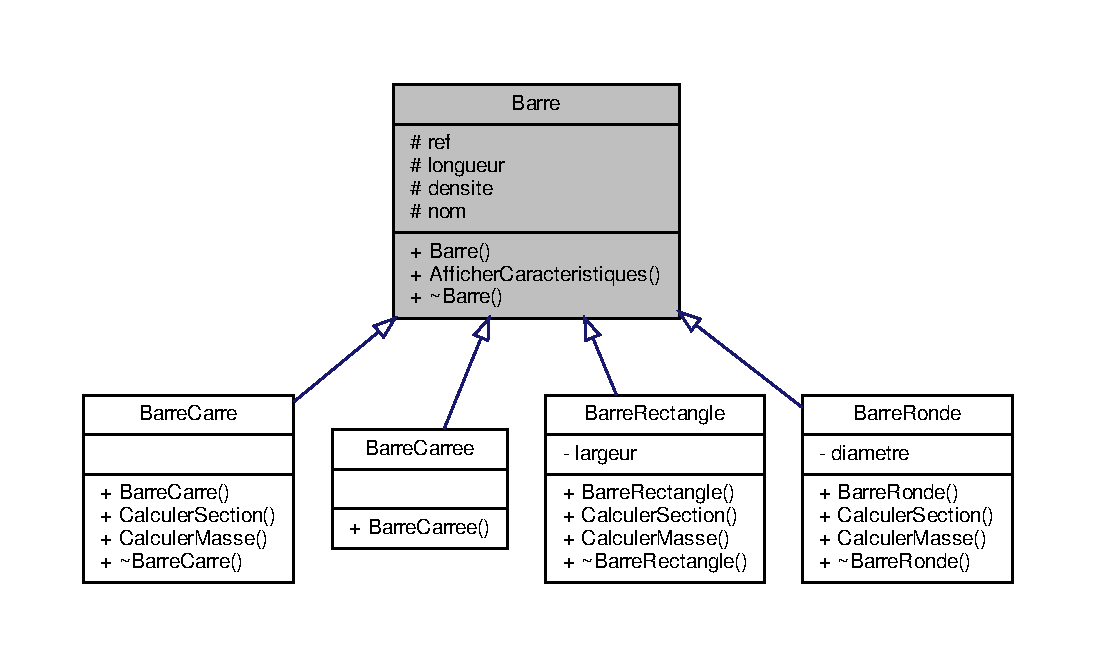
\includegraphics[width=350pt]{class_barre__inherit__graph}
\end{center}
\end{figure}


Graphe de collaboration de Barre\+:
\nopagebreak
\begin{figure}[H]
\begin{center}
\leavevmode
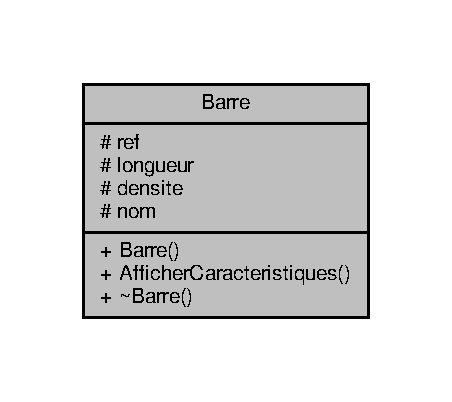
\includegraphics[width=217pt]{class_barre__coll__graph}
\end{center}
\end{figure}
\subsection*{Fonctions membres publiques}
\begin{DoxyCompactItemize}
\item 
\hyperlink{class_barre_aa47a7c516a56429545d7c63cf3a55bac}{Barre} (string \+\_\+ref, int \+\_\+longueur, float \+\_\+densite, string \+\_\+nom)
\begin{DoxyCompactList}\small\item\em \hyperlink{class_barre_aa47a7c516a56429545d7c63cf3a55bac}{Barre\+::\+Barre}. \end{DoxyCompactList}\item 
void \hyperlink{class_barre_a2e844be9d7c76a74d61cb14243a1bade}{Afficher\+Caracteristiques} ()
\begin{DoxyCompactList}\small\item\em \hyperlink{class_barre_a2e844be9d7c76a74d61cb14243a1bade}{Barre\+::\+Afficher\+Caracteristiques}. \end{DoxyCompactList}\item 
\hyperlink{class_barre_adc603c73952d56885cad1cc1acad578f}{$\sim$\+Barre} ()
\begin{DoxyCompactList}\small\item\em \hyperlink{class_barre_adc603c73952d56885cad1cc1acad578f}{Barre\+::$\sim$\+Barre}. \end{DoxyCompactList}\end{DoxyCompactItemize}
\subsection*{Attributs protégés}
\begin{DoxyCompactItemize}
\item 
string \hyperlink{class_barre_adc8a65b186d431c2c81f434d3d6973b1}{ref}
\item 
int \hyperlink{class_barre_a59f5637eaf9c15084deafab15f0de07d}{longueur}
\item 
float \hyperlink{class_barre_a1ed969f61782b23802f20ff7a5759f8d}{densite}
\item 
string \hyperlink{class_barre_a28ab665131a097ea05e175e461375362}{nom}
\end{DoxyCompactItemize}


\subsection{Documentation des constructeurs et destructeur}
\mbox{\Hypertarget{class_barre_aa47a7c516a56429545d7c63cf3a55bac}\label{class_barre_aa47a7c516a56429545d7c63cf3a55bac}} 
\index{Barre@{Barre}!Barre@{Barre}}
\index{Barre@{Barre}!Barre@{Barre}}
\subsubsection{\texorpdfstring{Barre()}{Barre()}}
{\footnotesize\ttfamily Barre\+::\+Barre (\begin{DoxyParamCaption}\item[{string}]{\+\_\+ref,  }\item[{int}]{\+\_\+longueur,  }\item[{float}]{\+\_\+densite,  }\item[{string}]{\+\_\+nom }\end{DoxyParamCaption})}



\hyperlink{class_barre_aa47a7c516a56429545d7c63cf3a55bac}{Barre\+::\+Barre}. 

Constructeur de la classe \hyperlink{class_barre}{Barre}, affecte les attributs de références, de longueur, de densité et le nom de la barre. 
\begin{DoxyParams}{Paramètres}
{\em \+\_\+ref} & indique une chaîne de caractère (la référence de la barre, ex.\+: \char`\"{}20-\/15\char`\"{}) \\
\hline
{\em \+\_\+longueur} & prend la valeur d\textquotesingle{}un entier \\
\hline
{\em \+\_\+densite} & prend la valeur d\textquotesingle{}un entier \\
\hline
{\em \+\_\+nom} & indique une chaîne de caractère (le nom de la barre, ex.\+: \char`\"{}\+Bronze\char`\"{}) \\
\hline
\end{DoxyParams}
\mbox{\Hypertarget{class_barre_adc603c73952d56885cad1cc1acad578f}\label{class_barre_adc603c73952d56885cad1cc1acad578f}} 
\index{Barre@{Barre}!````~Barre@{$\sim$\+Barre}}
\index{````~Barre@{$\sim$\+Barre}!Barre@{Barre}}
\subsubsection{\texorpdfstring{$\sim$\+Barre()}{~Barre()}}
{\footnotesize\ttfamily Barre\+::$\sim$\+Barre (\begin{DoxyParamCaption}{ }\end{DoxyParamCaption})}



\hyperlink{class_barre_adc603c73952d56885cad1cc1acad578f}{Barre\+::$\sim$\+Barre}. 

Destructeur de la classe \hyperlink{class_barre}{Barre} 

\subsection{Documentation des fonctions membres}
\mbox{\Hypertarget{class_barre_a2e844be9d7c76a74d61cb14243a1bade}\label{class_barre_a2e844be9d7c76a74d61cb14243a1bade}} 
\index{Barre@{Barre}!Afficher\+Caracteristiques@{Afficher\+Caracteristiques}}
\index{Afficher\+Caracteristiques@{Afficher\+Caracteristiques}!Barre@{Barre}}
\subsubsection{\texorpdfstring{Afficher\+Caracteristiques()}{AfficherCaracteristiques()}}
{\footnotesize\ttfamily void Barre\+::\+Afficher\+Caracteristiques (\begin{DoxyParamCaption}{ }\end{DoxyParamCaption})}



\hyperlink{class_barre_a2e844be9d7c76a74d61cb14243a1bade}{Barre\+::\+Afficher\+Caracteristiques}. 

Affiche les données contenues dans les variables 

\subsection{Documentation des données membres}
\mbox{\Hypertarget{class_barre_a1ed969f61782b23802f20ff7a5759f8d}\label{class_barre_a1ed969f61782b23802f20ff7a5759f8d}} 
\index{Barre@{Barre}!densite@{densite}}
\index{densite@{densite}!Barre@{Barre}}
\subsubsection{\texorpdfstring{densite}{densite}}
{\footnotesize\ttfamily float Barre\+::densite\hspace{0.3cm}{\ttfamily [protected]}}

\mbox{\Hypertarget{class_barre_a59f5637eaf9c15084deafab15f0de07d}\label{class_barre_a59f5637eaf9c15084deafab15f0de07d}} 
\index{Barre@{Barre}!longueur@{longueur}}
\index{longueur@{longueur}!Barre@{Barre}}
\subsubsection{\texorpdfstring{longueur}{longueur}}
{\footnotesize\ttfamily int Barre\+::longueur\hspace{0.3cm}{\ttfamily [protected]}}

\mbox{\Hypertarget{class_barre_a28ab665131a097ea05e175e461375362}\label{class_barre_a28ab665131a097ea05e175e461375362}} 
\index{Barre@{Barre}!nom@{nom}}
\index{nom@{nom}!Barre@{Barre}}
\subsubsection{\texorpdfstring{nom}{nom}}
{\footnotesize\ttfamily string Barre\+::nom\hspace{0.3cm}{\ttfamily [protected]}}

\mbox{\Hypertarget{class_barre_adc8a65b186d431c2c81f434d3d6973b1}\label{class_barre_adc8a65b186d431c2c81f434d3d6973b1}} 
\index{Barre@{Barre}!ref@{ref}}
\index{ref@{ref}!Barre@{Barre}}
\subsubsection{\texorpdfstring{ref}{ref}}
{\footnotesize\ttfamily string Barre\+::ref\hspace{0.3cm}{\ttfamily [protected]}}



La documentation de cette classe a été générée à partir des fichiers suivants \+:\begin{DoxyCompactItemize}
\item 
\hyperlink{barre_8h}{barre.\+h}\item 
\hyperlink{barre_8cpp}{barre.\+cpp}\end{DoxyCompactItemize}

\hypertarget{class_barre_carre}{}\section{Référence de la classe Barre\+Carre}
\label{class_barre_carre}\index{Barre\+Carre@{Barre\+Carre}}


{\ttfamily \#include $<$barrecarre.\+h$>$}



Graphe d\textquotesingle{}héritage de Barre\+Carre\+:
\nopagebreak
\begin{figure}[H]
\begin{center}
\leavevmode
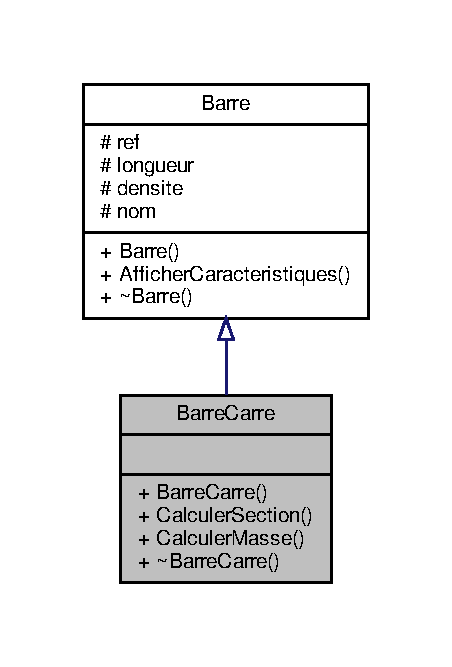
\includegraphics[width=217pt]{class_barre_carre__inherit__graph}
\end{center}
\end{figure}


Graphe de collaboration de Barre\+Carre\+:
\nopagebreak
\begin{figure}[H]
\begin{center}
\leavevmode
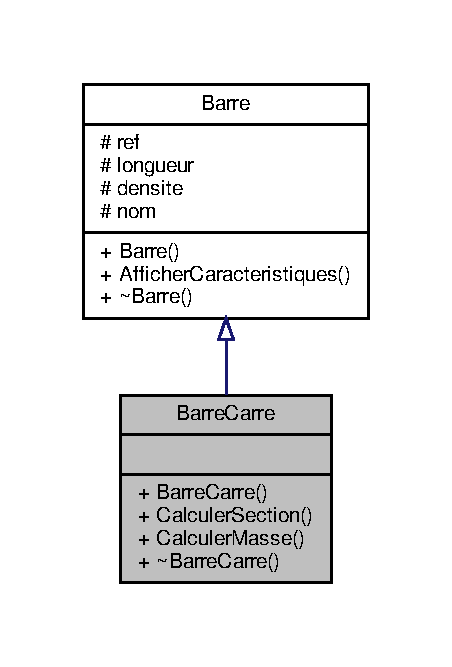
\includegraphics[width=217pt]{class_barre_carre__coll__graph}
\end{center}
\end{figure}
\subsection*{Fonctions membres publiques}
\begin{DoxyCompactItemize}
\item 
\hyperlink{class_barre_carre_ac0467aa6898dc560bee6d711b214da38}{Barre\+Carre} (string \+\_\+ref, int \+\_\+longueur, float \+\_\+densite, string \+\_\+nom)
\begin{DoxyCompactList}\small\item\em \hyperlink{class_barre_carre_ac0467aa6898dc560bee6d711b214da38}{Barre\+Carre\+::\+Barre\+Carre}. \end{DoxyCompactList}\item 
float \hyperlink{class_barre_carre_a521fa890549009143b4cd1fc0d20ba47}{Calculer\+Section} ()
\begin{DoxyCompactList}\small\item\em \hyperlink{class_barre_a2e844be9d7c76a74d61cb14243a1bade}{Barre\+::\+Afficher\+Caracteristiques}. \end{DoxyCompactList}\item 
float \hyperlink{class_barre_carre_ad290f96b7657082e3995c091a41a7a74}{Calculer\+Masse} ()
\begin{DoxyCompactList}\small\item\em \hyperlink{class_barre_carre_ad290f96b7657082e3995c091a41a7a74}{Barre\+Carre\+::\+Calculer\+Masse}. \end{DoxyCompactList}\item 
\hyperlink{class_barre_carre_a82339da142c13e06c3e464612dce0a42}{$\sim$\+Barre\+Carre} ()
\begin{DoxyCompactList}\small\item\em \hyperlink{class_barre_adc603c73952d56885cad1cc1acad578f}{Barre\+::$\sim$\+Barre}. \end{DoxyCompactList}\end{DoxyCompactItemize}
\subsection*{Membres hérités additionnels}


\subsection{Documentation des constructeurs et destructeur}
\mbox{\Hypertarget{class_barre_carre_ac0467aa6898dc560bee6d711b214da38}\label{class_barre_carre_ac0467aa6898dc560bee6d711b214da38}} 
\index{Barre\+Carre@{Barre\+Carre}!Barre\+Carre@{Barre\+Carre}}
\index{Barre\+Carre@{Barre\+Carre}!Barre\+Carre@{Barre\+Carre}}
\subsubsection{\texorpdfstring{Barre\+Carre()}{BarreCarre()}}
{\footnotesize\ttfamily Barre\+Carre\+::\+Barre\+Carre (\begin{DoxyParamCaption}\item[{string}]{\+\_\+ref,  }\item[{int}]{\+\_\+longueur,  }\item[{float}]{\+\_\+densite,  }\item[{string}]{\+\_\+nom }\end{DoxyParamCaption})}



\hyperlink{class_barre_carre_ac0467aa6898dc560bee6d711b214da38}{Barre\+Carre\+::\+Barre\+Carre}. 

Constructeur de la classe \hyperlink{class_barre_carre}{Barre\+Carre} 
\begin{DoxyParams}{Paramètres}
{\em \+\_\+ref} & indique une chaîne de caractère (la référence de la barre, ex.\+: \char`\"{}20-\/15\char`\"{}) \\
\hline
{\em \+\_\+longueur} & prend la valeur d\textquotesingle{}un entier \\
\hline
{\em \+\_\+densite} & prend la valeur d\textquotesingle{}un entier \\
\hline
{\em \+\_\+nom} & indique une chaîne de caractère (le nom de la barre, ex.\+: \char`\"{}\+Bronze\char`\"{}) \\
\hline
\end{DoxyParams}
\mbox{\Hypertarget{class_barre_carre_a82339da142c13e06c3e464612dce0a42}\label{class_barre_carre_a82339da142c13e06c3e464612dce0a42}} 
\index{Barre\+Carre@{Barre\+Carre}!````~Barre\+Carre@{$\sim$\+Barre\+Carre}}
\index{````~Barre\+Carre@{$\sim$\+Barre\+Carre}!Barre\+Carre@{Barre\+Carre}}
\subsubsection{\texorpdfstring{$\sim$\+Barre\+Carre()}{~BarreCarre()}}
{\footnotesize\ttfamily Barre\+Carre\+::$\sim$\+Barre\+Carre (\begin{DoxyParamCaption}{ }\end{DoxyParamCaption})}



\hyperlink{class_barre_adc603c73952d56885cad1cc1acad578f}{Barre\+::$\sim$\+Barre}. 

Destructeur de la classe \hyperlink{class_barre_carre}{Barre\+Carre} 

\subsection{Documentation des fonctions membres}
\mbox{\Hypertarget{class_barre_carre_ad290f96b7657082e3995c091a41a7a74}\label{class_barre_carre_ad290f96b7657082e3995c091a41a7a74}} 
\index{Barre\+Carre@{Barre\+Carre}!Calculer\+Masse@{Calculer\+Masse}}
\index{Calculer\+Masse@{Calculer\+Masse}!Barre\+Carre@{Barre\+Carre}}
\subsubsection{\texorpdfstring{Calculer\+Masse()}{CalculerMasse()}}
{\footnotesize\ttfamily float Barre\+Carre\+::\+Calculer\+Masse (\begin{DoxyParamCaption}{ }\end{DoxyParamCaption})}



\hyperlink{class_barre_carre_ad290f96b7657082e3995c091a41a7a74}{Barre\+Carre\+::\+Calculer\+Masse}. 

Renvoi le calcul de la masse de la barre \mbox{\Hypertarget{class_barre_carre_a521fa890549009143b4cd1fc0d20ba47}\label{class_barre_carre_a521fa890549009143b4cd1fc0d20ba47}} 
\index{Barre\+Carre@{Barre\+Carre}!Calculer\+Section@{Calculer\+Section}}
\index{Calculer\+Section@{Calculer\+Section}!Barre\+Carre@{Barre\+Carre}}
\subsubsection{\texorpdfstring{Calculer\+Section()}{CalculerSection()}}
{\footnotesize\ttfamily float Barre\+Carre\+::\+Calculer\+Section (\begin{DoxyParamCaption}{ }\end{DoxyParamCaption})}



\hyperlink{class_barre_a2e844be9d7c76a74d61cb14243a1bade}{Barre\+::\+Afficher\+Caracteristiques}. 

Renvoi le calcul de la section (aire) de la barre 

La documentation de cette classe a été générée à partir des fichiers suivants \+:\begin{DoxyCompactItemize}
\item 
\hyperlink{barrecarre_8h}{barrecarre.\+h}\item 
\hyperlink{barrecarre_8cpp}{barrecarre.\+cpp}\end{DoxyCompactItemize}

\hypertarget{class_barre_carree}{}\section{Référence de la classe Barre\+Carree}
\label{class_barre_carree}\index{Barre\+Carree@{Barre\+Carree}}


{\ttfamily \#include $<$barrecarree.\+h$>$}



Graphe d\textquotesingle{}héritage de Barre\+Carree\+:
\nopagebreak
\begin{figure}[H]
\begin{center}
\leavevmode
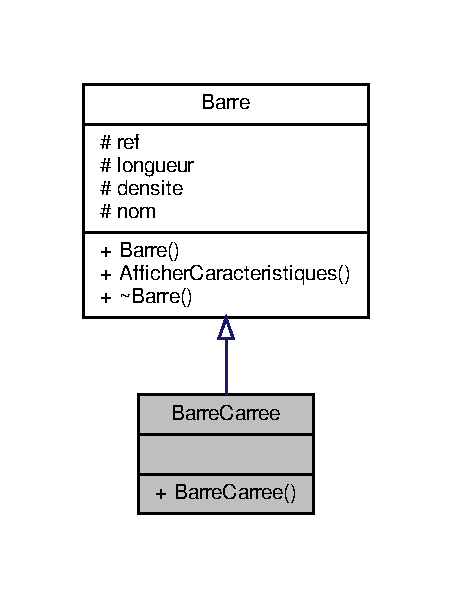
\includegraphics[width=217pt]{class_barre_carree__inherit__graph}
\end{center}
\end{figure}


Graphe de collaboration de Barre\+Carree\+:
\nopagebreak
\begin{figure}[H]
\begin{center}
\leavevmode
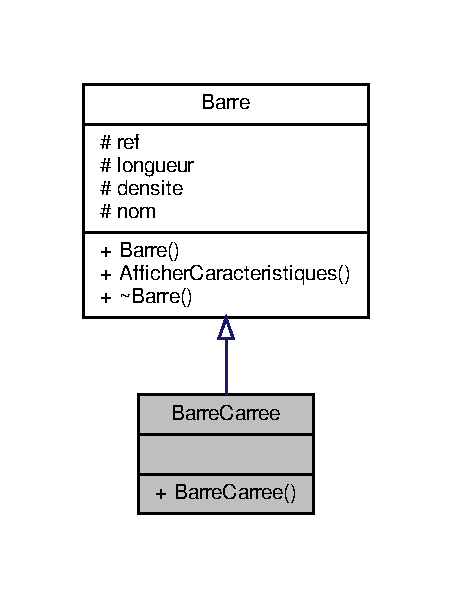
\includegraphics[width=217pt]{class_barre_carree__coll__graph}
\end{center}
\end{figure}
\subsection*{Fonctions membres publiques}
\begin{DoxyCompactItemize}
\item 
\hyperlink{class_barre_carree_a1fee50f3a72acb83aaf036024b872447}{Barre\+Carree} ()
\end{DoxyCompactItemize}
\subsection*{Membres hérités additionnels}


\subsection{Documentation des constructeurs et destructeur}
\mbox{\Hypertarget{class_barre_carree_a1fee50f3a72acb83aaf036024b872447}\label{class_barre_carree_a1fee50f3a72acb83aaf036024b872447}} 
\index{Barre\+Carree@{Barre\+Carree}!Barre\+Carree@{Barre\+Carree}}
\index{Barre\+Carree@{Barre\+Carree}!Barre\+Carree@{Barre\+Carree}}
\subsubsection{\texorpdfstring{Barre\+Carree()}{BarreCarree()}}
{\footnotesize\ttfamily Barre\+Carree\+::\+Barre\+Carree (\begin{DoxyParamCaption}{ }\end{DoxyParamCaption})}



La documentation de cette classe a été générée à partir des fichiers suivants \+:\begin{DoxyCompactItemize}
\item 
\hyperlink{barrecarree_8h}{barrecarree.\+h}\item 
\hyperlink{barrecarree_8cpp}{barrecarree.\+cpp}\end{DoxyCompactItemize}

\hypertarget{class_barre_rectangle}{}\section{Référence de la classe Barre\+Rectangle}
\label{class_barre_rectangle}\index{Barre\+Rectangle@{Barre\+Rectangle}}


{\ttfamily \#include $<$barrerectangle.\+h$>$}



Graphe d\textquotesingle{}héritage de Barre\+Rectangle\+:
\nopagebreak
\begin{figure}[H]
\begin{center}
\leavevmode
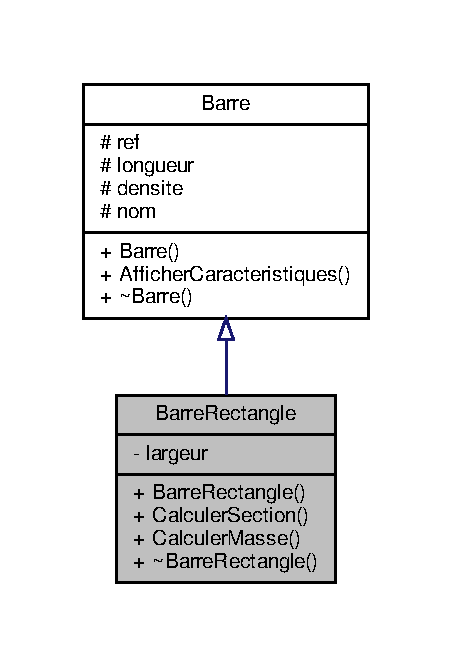
\includegraphics[width=217pt]{class_barre_rectangle__inherit__graph}
\end{center}
\end{figure}


Graphe de collaboration de Barre\+Rectangle\+:
\nopagebreak
\begin{figure}[H]
\begin{center}
\leavevmode
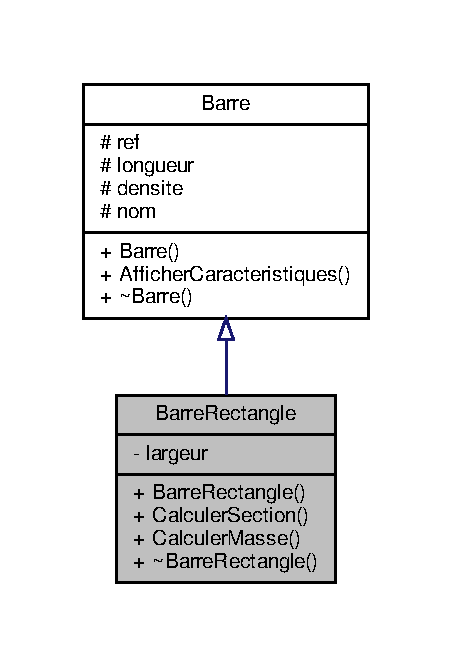
\includegraphics[width=217pt]{class_barre_rectangle__coll__graph}
\end{center}
\end{figure}
\subsection*{Fonctions membres publiques}
\begin{DoxyCompactItemize}
\item 
\hyperlink{class_barre_rectangle_ac11537dbce113614362ff8e67187504d}{Barre\+Rectangle} (string \+\_\+ref, int \+\_\+longueur, int \+\_\+largeur, float \+\_\+densite, string \+\_\+nom)
\begin{DoxyCompactList}\small\item\em \hyperlink{class_barre_rectangle_ac11537dbce113614362ff8e67187504d}{Barre\+Rectangle\+::\+Barre\+Rectangle}. \end{DoxyCompactList}\item 
float \hyperlink{class_barre_rectangle_aca359a79b9e74a94867ccaa4341f51ae}{Calculer\+Section} ()
\begin{DoxyCompactList}\small\item\em \hyperlink{class_barre_rectangle_aca359a79b9e74a94867ccaa4341f51ae}{Barre\+Rectangle\+::\+Calculer\+Section}. \end{DoxyCompactList}\item 
float \hyperlink{class_barre_rectangle_a9edb62e31a33790146eb0fd2b3fd7e4e}{Calculer\+Masse} ()
\begin{DoxyCompactList}\small\item\em \hyperlink{class_barre_rectangle_a9edb62e31a33790146eb0fd2b3fd7e4e}{Barre\+Rectangle\+::\+Calculer\+Masse}. \end{DoxyCompactList}\item 
\hyperlink{class_barre_rectangle_aaf9fee36e7a6b914af9fc0bff25674e4}{$\sim$\+Barre\+Rectangle} ()
\begin{DoxyCompactList}\small\item\em \hyperlink{class_barre_rectangle_aaf9fee36e7a6b914af9fc0bff25674e4}{Barre\+Rectangle\+::$\sim$\+Barre\+Rectangle}. \end{DoxyCompactList}\end{DoxyCompactItemize}
\subsection*{Attributs privés}
\begin{DoxyCompactItemize}
\item 
int \hyperlink{class_barre_rectangle_a6805bad77d9cbdf787a911e0841d6d35}{largeur}
\end{DoxyCompactItemize}
\subsection*{Membres hérités additionnels}


\subsection{Documentation des constructeurs et destructeur}
\mbox{\Hypertarget{class_barre_rectangle_ac11537dbce113614362ff8e67187504d}\label{class_barre_rectangle_ac11537dbce113614362ff8e67187504d}} 
\index{Barre\+Rectangle@{Barre\+Rectangle}!Barre\+Rectangle@{Barre\+Rectangle}}
\index{Barre\+Rectangle@{Barre\+Rectangle}!Barre\+Rectangle@{Barre\+Rectangle}}
\subsubsection{\texorpdfstring{Barre\+Rectangle()}{BarreRectangle()}}
{\footnotesize\ttfamily Barre\+Rectangle\+::\+Barre\+Rectangle (\begin{DoxyParamCaption}\item[{string}]{\+\_\+ref,  }\item[{int}]{\+\_\+longueur,  }\item[{int}]{\+\_\+largeur,  }\item[{float}]{\+\_\+densite,  }\item[{string}]{\+\_\+nom }\end{DoxyParamCaption})}



\hyperlink{class_barre_rectangle_ac11537dbce113614362ff8e67187504d}{Barre\+Rectangle\+::\+Barre\+Rectangle}. 

constructeur de la classe \hyperlink{class_barre_rectangle}{Barre\+Rectangle} 
\begin{DoxyParams}{Paramètres}
{\em \+\_\+ref} & indique une chaîne de caractère (la référence de la barre, ex.\+: \char`\"{}20-\/15\char`\"{}) \\
\hline
{\em \+\_\+longueur} & prend la valeur d\textquotesingle{}un entier \\
\hline
{\em \+\_\+largeur} & prend la valeur d\textquotesingle{}un entier \\
\hline
{\em \+\_\+densite} & prend la valeur d\textquotesingle{}un entier \\
\hline
{\em \+\_\+nom} & indique une chaîne de caractère (le nom de la barre, ex.\+: \char`\"{}\+Bronze\char`\"{}) \\
\hline
\end{DoxyParams}
\mbox{\Hypertarget{class_barre_rectangle_aaf9fee36e7a6b914af9fc0bff25674e4}\label{class_barre_rectangle_aaf9fee36e7a6b914af9fc0bff25674e4}} 
\index{Barre\+Rectangle@{Barre\+Rectangle}!````~Barre\+Rectangle@{$\sim$\+Barre\+Rectangle}}
\index{````~Barre\+Rectangle@{$\sim$\+Barre\+Rectangle}!Barre\+Rectangle@{Barre\+Rectangle}}
\subsubsection{\texorpdfstring{$\sim$\+Barre\+Rectangle()}{~BarreRectangle()}}
{\footnotesize\ttfamily Barre\+Rectangle\+::$\sim$\+Barre\+Rectangle (\begin{DoxyParamCaption}{ }\end{DoxyParamCaption})}



\hyperlink{class_barre_rectangle_aaf9fee36e7a6b914af9fc0bff25674e4}{Barre\+Rectangle\+::$\sim$\+Barre\+Rectangle}. 

Destructeur de la classe \hyperlink{class_barre_rectangle}{Barre\+Rectangle} 

\subsection{Documentation des fonctions membres}
\mbox{\Hypertarget{class_barre_rectangle_a9edb62e31a33790146eb0fd2b3fd7e4e}\label{class_barre_rectangle_a9edb62e31a33790146eb0fd2b3fd7e4e}} 
\index{Barre\+Rectangle@{Barre\+Rectangle}!Calculer\+Masse@{Calculer\+Masse}}
\index{Calculer\+Masse@{Calculer\+Masse}!Barre\+Rectangle@{Barre\+Rectangle}}
\subsubsection{\texorpdfstring{Calculer\+Masse()}{CalculerMasse()}}
{\footnotesize\ttfamily float Barre\+Rectangle\+::\+Calculer\+Masse (\begin{DoxyParamCaption}{ }\end{DoxyParamCaption})}



\hyperlink{class_barre_rectangle_a9edb62e31a33790146eb0fd2b3fd7e4e}{Barre\+Rectangle\+::\+Calculer\+Masse}. 

Renvoi le calcul de la masse de la barre \mbox{\Hypertarget{class_barre_rectangle_aca359a79b9e74a94867ccaa4341f51ae}\label{class_barre_rectangle_aca359a79b9e74a94867ccaa4341f51ae}} 
\index{Barre\+Rectangle@{Barre\+Rectangle}!Calculer\+Section@{Calculer\+Section}}
\index{Calculer\+Section@{Calculer\+Section}!Barre\+Rectangle@{Barre\+Rectangle}}
\subsubsection{\texorpdfstring{Calculer\+Section()}{CalculerSection()}}
{\footnotesize\ttfamily float Barre\+Rectangle\+::\+Calculer\+Section (\begin{DoxyParamCaption}{ }\end{DoxyParamCaption})}



\hyperlink{class_barre_rectangle_aca359a79b9e74a94867ccaa4341f51ae}{Barre\+Rectangle\+::\+Calculer\+Section}. 

Renvoi le calcul de la section (aire) de la barre 

\subsection{Documentation des données membres}
\mbox{\Hypertarget{class_barre_rectangle_a6805bad77d9cbdf787a911e0841d6d35}\label{class_barre_rectangle_a6805bad77d9cbdf787a911e0841d6d35}} 
\index{Barre\+Rectangle@{Barre\+Rectangle}!largeur@{largeur}}
\index{largeur@{largeur}!Barre\+Rectangle@{Barre\+Rectangle}}
\subsubsection{\texorpdfstring{largeur}{largeur}}
{\footnotesize\ttfamily int Barre\+Rectangle\+::largeur\hspace{0.3cm}{\ttfamily [private]}}



La documentation de cette classe a été générée à partir des fichiers suivants \+:\begin{DoxyCompactItemize}
\item 
\hyperlink{barrerectangle_8h}{barrerectangle.\+h}\item 
\hyperlink{barrerectangle_8cpp}{barrerectangle.\+cpp}\end{DoxyCompactItemize}

\hypertarget{class_barre_ronde}{}\section{Référence de la classe Barre\+Ronde}
\label{class_barre_ronde}\index{Barre\+Ronde@{Barre\+Ronde}}


{\ttfamily \#include $<$barreronde.\+h$>$}



Graphe d\textquotesingle{}héritage de Barre\+Ronde\+:
\nopagebreak
\begin{figure}[H]
\begin{center}
\leavevmode
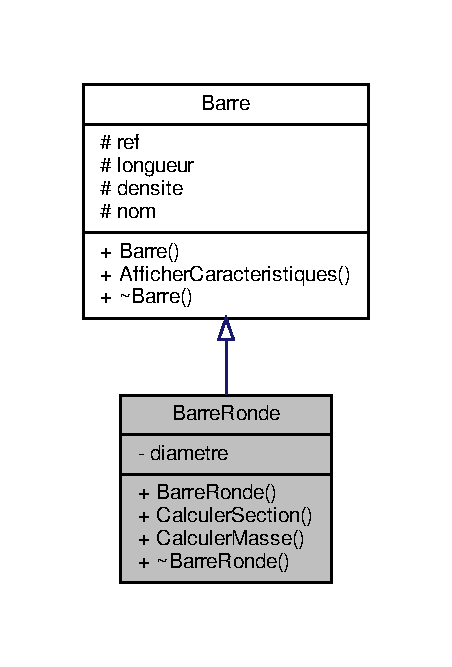
\includegraphics[width=217pt]{class_barre_ronde__inherit__graph}
\end{center}
\end{figure}


Graphe de collaboration de Barre\+Ronde\+:
\nopagebreak
\begin{figure}[H]
\begin{center}
\leavevmode
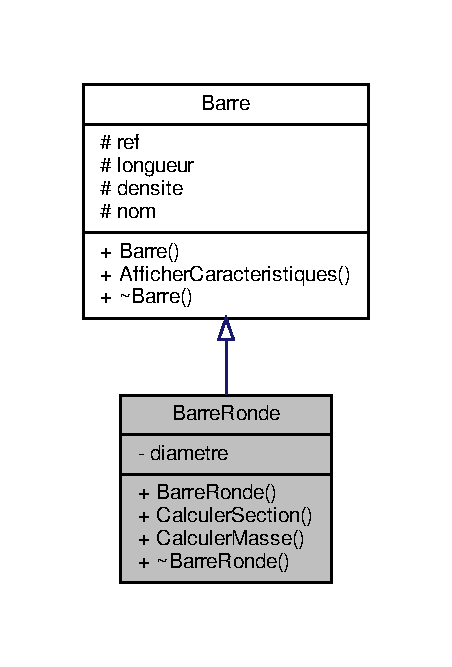
\includegraphics[width=217pt]{class_barre_ronde__coll__graph}
\end{center}
\end{figure}
\subsection*{Fonctions membres publiques}
\begin{DoxyCompactItemize}
\item 
\hyperlink{class_barre_ronde_a71f08d5ff38305f39ed7d6205941ec3e}{Barre\+Ronde} (string \+\_\+ref, int \+\_\+longueur, int \+\_\+diametre, float \+\_\+densite, string \+\_\+nom)
\begin{DoxyCompactList}\small\item\em \hyperlink{class_barre_ronde_a71f08d5ff38305f39ed7d6205941ec3e}{Barre\+Ronde\+::\+Barre\+Ronde}. \end{DoxyCompactList}\item 
double \hyperlink{class_barre_ronde_adc6f65b51c7ca244fb29f2ed4b9a6f91}{Calculer\+Section} ()
\begin{DoxyCompactList}\small\item\em \hyperlink{class_barre_ronde_adc6f65b51c7ca244fb29f2ed4b9a6f91}{Barre\+Ronde\+::\+Calculer\+Section}. \end{DoxyCompactList}\item 
float \hyperlink{class_barre_ronde_a450c58e2bfcb1300339f1c790740e5ad}{Calculer\+Masse} ()
\begin{DoxyCompactList}\small\item\em \hyperlink{class_barre_ronde_a450c58e2bfcb1300339f1c790740e5ad}{Barre\+Ronde\+::\+Calculer\+Masse}. \end{DoxyCompactList}\item 
\hyperlink{class_barre_ronde_aa62c3c350d2153aefcab64a20a6a795a}{$\sim$\+Barre\+Ronde} ()
\begin{DoxyCompactList}\small\item\em \hyperlink{class_barre_ronde_aa62c3c350d2153aefcab64a20a6a795a}{Barre\+Ronde\+::$\sim$\+Barre\+Ronde}. \end{DoxyCompactList}\end{DoxyCompactItemize}
\subsection*{Attributs privés}
\begin{DoxyCompactItemize}
\item 
int \hyperlink{class_barre_ronde_a2ad361c8aefdf0f7b25bbcbc1ec4c4ca}{diametre}
\end{DoxyCompactItemize}
\subsection*{Membres hérités additionnels}


\subsection{Documentation des constructeurs et destructeur}
\mbox{\Hypertarget{class_barre_ronde_a71f08d5ff38305f39ed7d6205941ec3e}\label{class_barre_ronde_a71f08d5ff38305f39ed7d6205941ec3e}} 
\index{Barre\+Ronde@{Barre\+Ronde}!Barre\+Ronde@{Barre\+Ronde}}
\index{Barre\+Ronde@{Barre\+Ronde}!Barre\+Ronde@{Barre\+Ronde}}
\subsubsection{\texorpdfstring{Barre\+Ronde()}{BarreRonde()}}
{\footnotesize\ttfamily Barre\+Ronde\+::\+Barre\+Ronde (\begin{DoxyParamCaption}\item[{string}]{\+\_\+ref,  }\item[{int}]{\+\_\+longueur,  }\item[{int}]{\+\_\+diametre,  }\item[{float}]{\+\_\+densite,  }\item[{string}]{\+\_\+nom }\end{DoxyParamCaption})}



\hyperlink{class_barre_ronde_a71f08d5ff38305f39ed7d6205941ec3e}{Barre\+Ronde\+::\+Barre\+Ronde}. 

constructeur de la classe \hyperlink{class_barre_ronde}{Barre\+Ronde} 
\begin{DoxyParams}{Paramètres}
{\em \+\_\+ref} & indique une chaîne de caractère (la référence de la barre, ex.\+: \char`\"{}20-\/15\char`\"{}) \\
\hline
{\em \+\_\+longueur} & prend la valeur d\textquotesingle{}un entier \\
\hline
{\em \+\_\+diametre} & prend la valeur d\textquotesingle{}un entier \\
\hline
{\em \+\_\+densite} & prend la valeur d\textquotesingle{}un entier \\
\hline
{\em \+\_\+nom} & indique une chaîne de caractère (le nom de la barre, ex.\+: \char`\"{}\+Bronze\char`\"{}) \\
\hline
\end{DoxyParams}
\mbox{\Hypertarget{class_barre_ronde_aa62c3c350d2153aefcab64a20a6a795a}\label{class_barre_ronde_aa62c3c350d2153aefcab64a20a6a795a}} 
\index{Barre\+Ronde@{Barre\+Ronde}!````~Barre\+Ronde@{$\sim$\+Barre\+Ronde}}
\index{````~Barre\+Ronde@{$\sim$\+Barre\+Ronde}!Barre\+Ronde@{Barre\+Ronde}}
\subsubsection{\texorpdfstring{$\sim$\+Barre\+Ronde()}{~BarreRonde()}}
{\footnotesize\ttfamily Barre\+Ronde\+::$\sim$\+Barre\+Ronde (\begin{DoxyParamCaption}{ }\end{DoxyParamCaption})}



\hyperlink{class_barre_ronde_aa62c3c350d2153aefcab64a20a6a795a}{Barre\+Ronde\+::$\sim$\+Barre\+Ronde}. 

Destructeur de la classe \hyperlink{class_barre_ronde}{Barre\+Ronde} 

\subsection{Documentation des fonctions membres}
\mbox{\Hypertarget{class_barre_ronde_a450c58e2bfcb1300339f1c790740e5ad}\label{class_barre_ronde_a450c58e2bfcb1300339f1c790740e5ad}} 
\index{Barre\+Ronde@{Barre\+Ronde}!Calculer\+Masse@{Calculer\+Masse}}
\index{Calculer\+Masse@{Calculer\+Masse}!Barre\+Ronde@{Barre\+Ronde}}
\subsubsection{\texorpdfstring{Calculer\+Masse()}{CalculerMasse()}}
{\footnotesize\ttfamily float Barre\+Ronde\+::\+Calculer\+Masse (\begin{DoxyParamCaption}{ }\end{DoxyParamCaption})}



\hyperlink{class_barre_ronde_a450c58e2bfcb1300339f1c790740e5ad}{Barre\+Ronde\+::\+Calculer\+Masse}. 

Renvoi le calcul de la masse de la barre \mbox{\Hypertarget{class_barre_ronde_adc6f65b51c7ca244fb29f2ed4b9a6f91}\label{class_barre_ronde_adc6f65b51c7ca244fb29f2ed4b9a6f91}} 
\index{Barre\+Ronde@{Barre\+Ronde}!Calculer\+Section@{Calculer\+Section}}
\index{Calculer\+Section@{Calculer\+Section}!Barre\+Ronde@{Barre\+Ronde}}
\subsubsection{\texorpdfstring{Calculer\+Section()}{CalculerSection()}}
{\footnotesize\ttfamily double Barre\+Ronde\+::\+Calculer\+Section (\begin{DoxyParamCaption}{ }\end{DoxyParamCaption})}



\hyperlink{class_barre_ronde_adc6f65b51c7ca244fb29f2ed4b9a6f91}{Barre\+Ronde\+::\+Calculer\+Section}. 

Renvoi le calcul de la section (aire) de la barre 

\subsection{Documentation des données membres}
\mbox{\Hypertarget{class_barre_ronde_a2ad361c8aefdf0f7b25bbcbc1ec4c4ca}\label{class_barre_ronde_a2ad361c8aefdf0f7b25bbcbc1ec4c4ca}} 
\index{Barre\+Ronde@{Barre\+Ronde}!diametre@{diametre}}
\index{diametre@{diametre}!Barre\+Ronde@{Barre\+Ronde}}
\subsubsection{\texorpdfstring{diametre}{diametre}}
{\footnotesize\ttfamily int Barre\+Ronde\+::diametre\hspace{0.3cm}{\ttfamily [private]}}



La documentation de cette classe a été générée à partir des fichiers suivants \+:\begin{DoxyCompactItemize}
\item 
\hyperlink{barreronde_8h}{barreronde.\+h}\item 
\hyperlink{barreronde_8cpp}{barreronde.\+cpp}\end{DoxyCompactItemize}

\chapter{Documentation des fichiers}
\hypertarget{barre_8cpp}{}\section{Référence du fichier barre.\+cpp}
\label{barre_8cpp}\index{barre.\+cpp@{barre.\+cpp}}


implémentation de la classe \hyperlink{class_barre}{Barre}  


{\ttfamily \#include \char`\"{}barre.\+h\char`\"{}}\newline
Graphe des dépendances par inclusion de barre.\+cpp\+:
\nopagebreak
\begin{figure}[H]
\begin{center}
\leavevmode
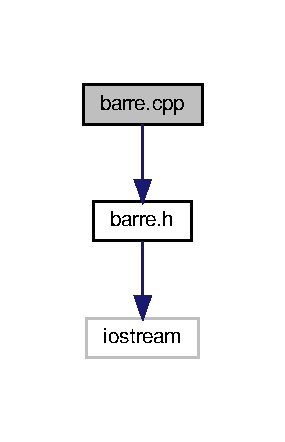
\includegraphics[width=137pt]{barre_8cpp__incl}
\end{center}
\end{figure}


\subsection{Description détaillée}
implémentation de la classe \hyperlink{class_barre}{Barre} 

\begin{DoxyVersion}{Version}
1.\+1 
\end{DoxyVersion}
\begin{DoxyAuthor}{Auteur}
Antoine C\+H\+E\+V\+R\+EL 
\end{DoxyAuthor}
\begin{DoxyDate}{Date}
20 septembre 2019 
\end{DoxyDate}

\hypertarget{barre_8h}{}\section{Référence du fichier barre.\+h}
\label{barre_8h}\index{barre.\+h@{barre.\+h}}


Définition de la classe \hyperlink{class_barre}{Barre}.  


{\ttfamily \#include $<$iostream$>$}\newline
Graphe des dépendances par inclusion de barre.\+h\+:
\nopagebreak
\begin{figure}[H]
\begin{center}
\leavevmode
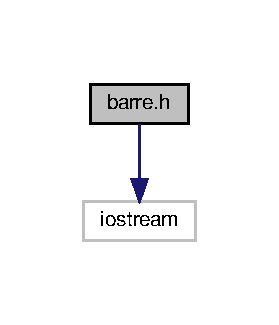
\includegraphics[width=134pt]{barre_8h__incl}
\end{center}
\end{figure}
Ce graphe montre quels fichiers incluent directement ou indirectement ce fichier \+:
\nopagebreak
\begin{figure}[H]
\begin{center}
\leavevmode
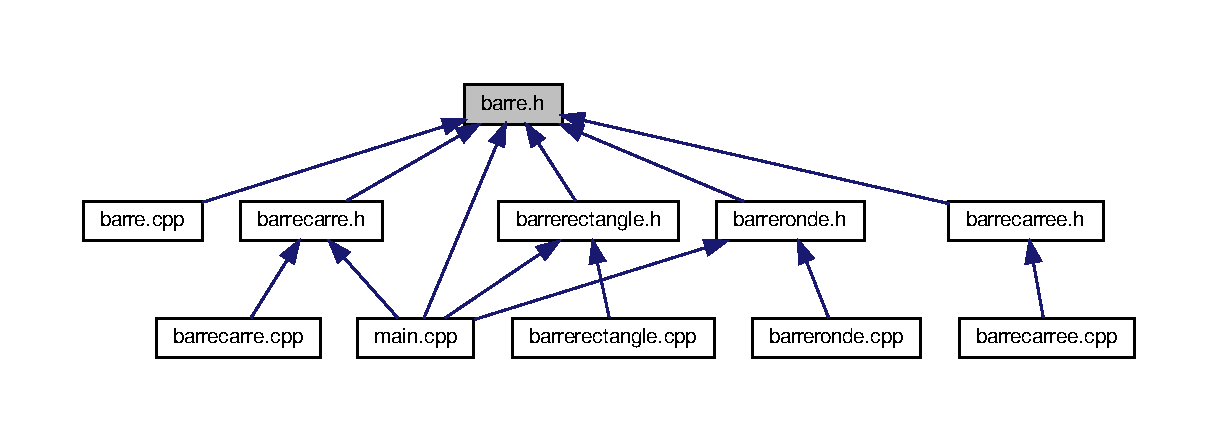
\includegraphics[width=350pt]{barre_8h__dep__incl}
\end{center}
\end{figure}
\subsection*{Classes}
\begin{DoxyCompactItemize}
\item 
class \hyperlink{class_barre}{Barre}
\end{DoxyCompactItemize}


\subsection{Description détaillée}
Définition de la classe \hyperlink{class_barre}{Barre}. 

\begin{DoxyVersion}{Version}
1.\+1 
\end{DoxyVersion}
\begin{DoxyAuthor}{Auteur}
Antoine C\+H\+E\+V\+R\+EL 
\end{DoxyAuthor}
\begin{DoxyDate}{Date}
20 septembre 2019 
\end{DoxyDate}

\hypertarget{barrecarre_8cpp}{}\section{Référence du fichier barrecarre.\+cpp}
\label{barrecarre_8cpp}\index{barrecarre.\+cpp@{barrecarre.\+cpp}}


implémentation de la classe \hyperlink{class_barre_carre}{Barre\+Carre}  


{\ttfamily \#include \char`\"{}barrecarre.\+h\char`\"{}}\newline
Graphe des dépendances par inclusion de barrecarre.\+cpp\+:
\nopagebreak
\begin{figure}[H]
\begin{center}
\leavevmode
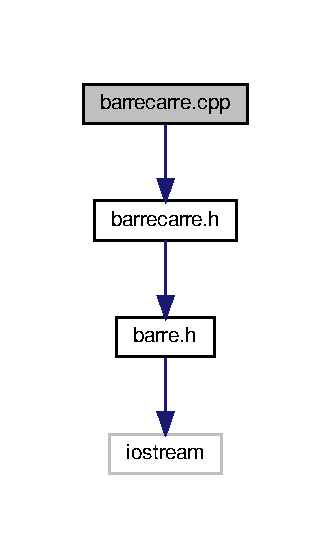
\includegraphics[width=159pt]{barrecarre_8cpp__incl}
\end{center}
\end{figure}


\subsection{Description détaillée}
implémentation de la classe \hyperlink{class_barre_carre}{Barre\+Carre} 

\begin{DoxyVersion}{Version}
1.\+1 
\end{DoxyVersion}
\begin{DoxyAuthor}{Auteur}
Antoine C\+H\+E\+V\+R\+EL 
\end{DoxyAuthor}
\begin{DoxyDate}{Date}
20 septembre 2019 
\end{DoxyDate}

\hypertarget{barrecarre_8h}{}\section{Référence du fichier barrecarre.\+h}
\label{barrecarre_8h}\index{barrecarre.\+h@{barrecarre.\+h}}


Définition de la classe \hyperlink{class_barre_carre}{Barre\+Carre}.  


{\ttfamily \#include \char`\"{}barre.\+h\char`\"{}}\newline
Graphe des dépendances par inclusion de barrecarre.\+h\+:
\nopagebreak
\begin{figure}[H]
\begin{center}
\leavevmode
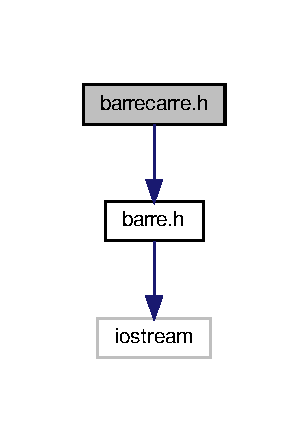
\includegraphics[width=148pt]{barrecarre_8h__incl}
\end{center}
\end{figure}
Ce graphe montre quels fichiers incluent directement ou indirectement ce fichier \+:
\nopagebreak
\begin{figure}[H]
\begin{center}
\leavevmode
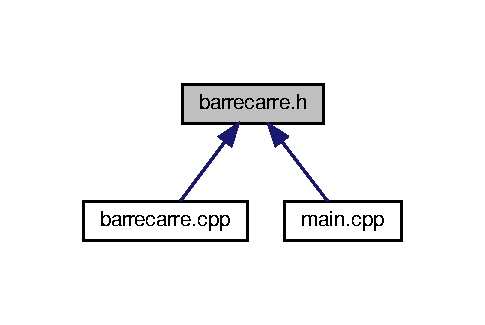
\includegraphics[width=233pt]{barrecarre_8h__dep__incl}
\end{center}
\end{figure}
\subsection*{Classes}
\begin{DoxyCompactItemize}
\item 
class \hyperlink{class_barre_carre}{Barre\+Carre}
\end{DoxyCompactItemize}


\subsection{Description détaillée}
Définition de la classe \hyperlink{class_barre_carre}{Barre\+Carre}. 

\begin{DoxyVersion}{Version}
1.\+1 
\end{DoxyVersion}
\begin{DoxyAuthor}{Auteur}
Antoine C\+H\+E\+V\+R\+EL 
\end{DoxyAuthor}
\begin{DoxyDate}{Date}
20 septembre 2019 
\end{DoxyDate}

\hypertarget{barrecarree_8cpp}{}\section{Référence du fichier barrecarree.\+cpp}
\label{barrecarree_8cpp}\index{barrecarree.\+cpp@{barrecarree.\+cpp}}
{\ttfamily \#include \char`\"{}barrecarree.\+h\char`\"{}}\newline
Graphe des dépendances par inclusion de barrecarree.\+cpp\+:
\nopagebreak
\begin{figure}[H]
\begin{center}
\leavevmode
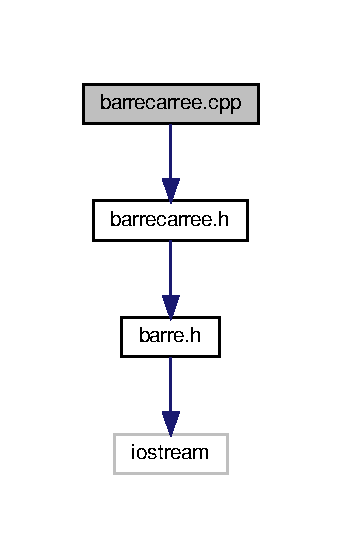
\includegraphics[width=164pt]{barrecarree_8cpp__incl}
\end{center}
\end{figure}

\hypertarget{barrecarree_8h}{}\section{Référence du fichier barrecarree.\+h}
\label{barrecarree_8h}\index{barrecarree.\+h@{barrecarree.\+h}}
{\ttfamily \#include \char`\"{}barre.\+h\char`\"{}}\newline
Graphe des dépendances par inclusion de barrecarree.\+h\+:
\nopagebreak
\begin{figure}[H]
\begin{center}
\leavevmode
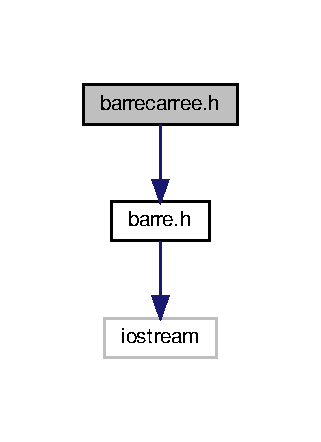
\includegraphics[width=154pt]{barrecarree_8h__incl}
\end{center}
\end{figure}
Ce graphe montre quels fichiers incluent directement ou indirectement ce fichier \+:
\nopagebreak
\begin{figure}[H]
\begin{center}
\leavevmode
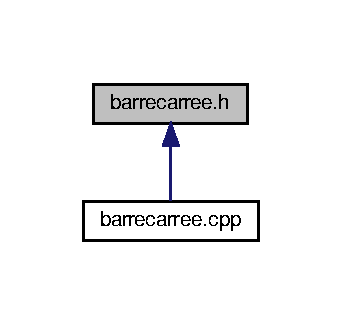
\includegraphics[width=164pt]{barrecarree_8h__dep__incl}
\end{center}
\end{figure}
\subsection*{Classes}
\begin{DoxyCompactItemize}
\item 
class \hyperlink{class_barre_carree}{Barre\+Carree}
\end{DoxyCompactItemize}

\hypertarget{barrerectangle_8cpp}{}\section{Référence du fichier barrerectangle.\+cpp}
\label{barrerectangle_8cpp}\index{barrerectangle.\+cpp@{barrerectangle.\+cpp}}


implémentation de la classe \hyperlink{class_barre_rectangle}{Barre\+Rectangle}  


{\ttfamily \#include \char`\"{}barrerectangle.\+h\char`\"{}}\newline
Graphe des dépendances par inclusion de barrerectangle.\+cpp\+:
\nopagebreak
\begin{figure}[H]
\begin{center}
\leavevmode
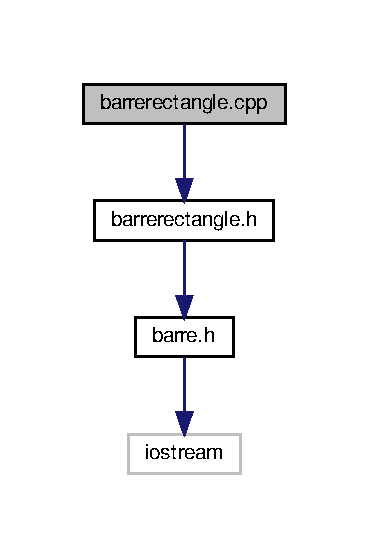
\includegraphics[width=177pt]{barrerectangle_8cpp__incl}
\end{center}
\end{figure}


\subsection{Description détaillée}
implémentation de la classe \hyperlink{class_barre_rectangle}{Barre\+Rectangle} 

\begin{DoxyVersion}{Version}
1.\+1 
\end{DoxyVersion}
\begin{DoxyAuthor}{Auteur}
Antoine C\+H\+E\+V\+R\+EL 
\end{DoxyAuthor}
\begin{DoxyDate}{Date}
20 septembre 2019 
\end{DoxyDate}

\hypertarget{barrerectangle_8h}{}\section{Référence du fichier barrerectangle.\+h}
\label{barrerectangle_8h}\index{barrerectangle.\+h@{barrerectangle.\+h}}


Définition de la classe \hyperlink{class_barre_rectangle}{Barre\+Rectangle}.  


{\ttfamily \#include \char`\"{}barre.\+h\char`\"{}}\newline
Graphe des dépendances par inclusion de barrerectangle.\+h\+:
\nopagebreak
\begin{figure}[H]
\begin{center}
\leavevmode
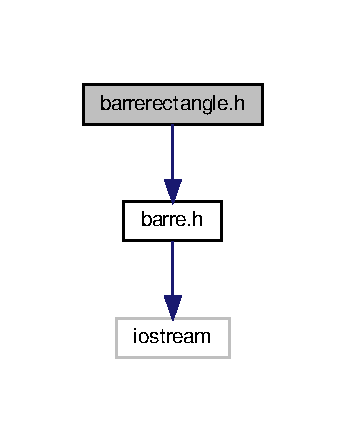
\includegraphics[width=166pt]{barrerectangle_8h__incl}
\end{center}
\end{figure}
Ce graphe montre quels fichiers incluent directement ou indirectement ce fichier \+:
\nopagebreak
\begin{figure}[H]
\begin{center}
\leavevmode
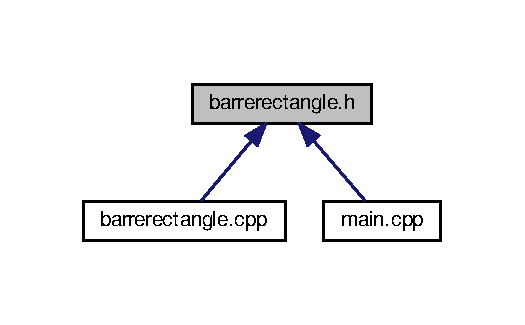
\includegraphics[width=252pt]{barrerectangle_8h__dep__incl}
\end{center}
\end{figure}
\subsection*{Classes}
\begin{DoxyCompactItemize}
\item 
class \hyperlink{class_barre_rectangle}{Barre\+Rectangle}
\end{DoxyCompactItemize}


\subsection{Description détaillée}
Définition de la classe \hyperlink{class_barre_rectangle}{Barre\+Rectangle}. 

\begin{DoxyVersion}{Version}
1.\+1 
\end{DoxyVersion}
\begin{DoxyAuthor}{Auteur}
Antoine C\+H\+E\+V\+R\+EL 
\end{DoxyAuthor}
\begin{DoxyDate}{Date}
20 septembre 2019 
\end{DoxyDate}

\hypertarget{barreronde_8cpp}{}\section{Référence du fichier barreronde.\+cpp}
\label{barreronde_8cpp}\index{barreronde.\+cpp@{barreronde.\+cpp}}


implémentation de la classe \hyperlink{class_barre_ronde}{Barre\+Ronde}  


{\ttfamily \#include \char`\"{}barreronde.\+h\char`\"{}}\newline
{\ttfamily \#include $<$math.\+h$>$}\newline
Graphe des dépendances par inclusion de barreronde.\+cpp\+:
\nopagebreak
\begin{figure}[H]
\begin{center}
\leavevmode
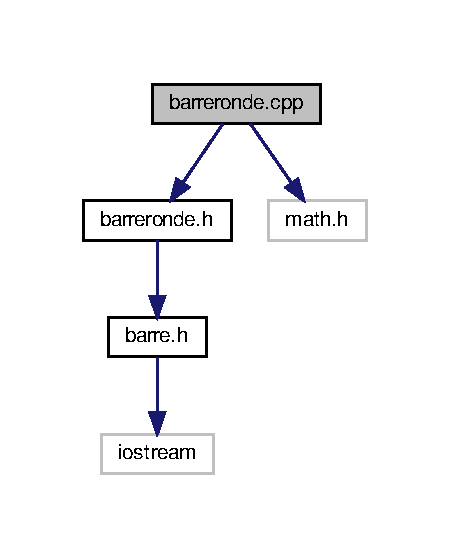
\includegraphics[width=216pt]{barreronde_8cpp__incl}
\end{center}
\end{figure}


\subsection{Description détaillée}
implémentation de la classe \hyperlink{class_barre_ronde}{Barre\+Ronde} 

\begin{DoxyVersion}{Version}
1.\+1 
\end{DoxyVersion}
\begin{DoxyAuthor}{Auteur}
Antoine C\+H\+E\+V\+R\+EL 
\end{DoxyAuthor}
\begin{DoxyDate}{Date}
20 septembre 2019 
\end{DoxyDate}

\hypertarget{barreronde_8h}{}\section{Référence du fichier barreronde.\+h}
\label{barreronde_8h}\index{barreronde.\+h@{barreronde.\+h}}


Définition de la classe \hyperlink{class_barre_ronde}{Barre\+Ronde}.  


{\ttfamily \#include \char`\"{}barre.\+h\char`\"{}}\newline
Graphe des dépendances par inclusion de barreronde.\+h\+:
\nopagebreak
\begin{figure}[H]
\begin{center}
\leavevmode
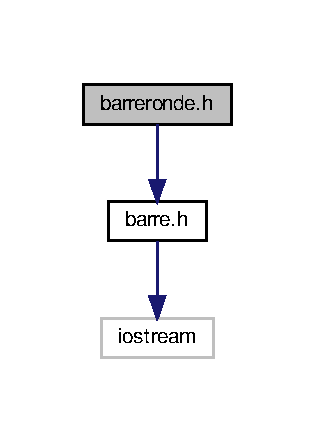
\includegraphics[width=151pt]{barreronde_8h__incl}
\end{center}
\end{figure}
Ce graphe montre quels fichiers incluent directement ou indirectement ce fichier \+:
\nopagebreak
\begin{figure}[H]
\begin{center}
\leavevmode
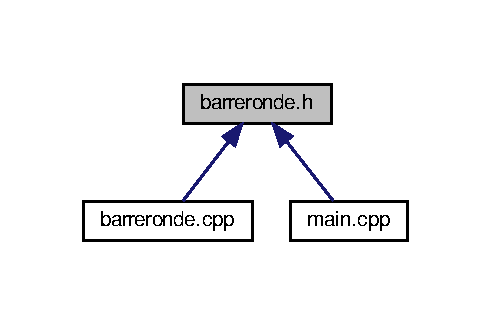
\includegraphics[width=236pt]{barreronde_8h__dep__incl}
\end{center}
\end{figure}
\subsection*{Classes}
\begin{DoxyCompactItemize}
\item 
class \hyperlink{class_barre_ronde}{Barre\+Ronde}
\end{DoxyCompactItemize}


\subsection{Description détaillée}
Définition de la classe \hyperlink{class_barre_ronde}{Barre\+Ronde}. 

\begin{DoxyVersion}{Version}
1.\+1 
\end{DoxyVersion}
\begin{DoxyAuthor}{Auteur}
Antoine C\+H\+E\+V\+R\+EL 
\end{DoxyAuthor}
\begin{DoxyDate}{Date}
20 septembre 2019 
\end{DoxyDate}

\hypertarget{main_8cpp}{}\section{Référence du fichier main.\+cpp}
\label{main_8cpp}\index{main.\+cpp@{main.\+cpp}}
{\ttfamily \#include $<$iostream$>$}\newline
{\ttfamily \#include \char`\"{}barre.\+h\char`\"{}}\newline
{\ttfamily \#include \char`\"{}barrecarre.\+h\char`\"{}}\newline
{\ttfamily \#include \char`\"{}barrerectangle.\+h\char`\"{}}\newline
{\ttfamily \#include \char`\"{}barreronde.\+h\char`\"{}}\newline
Graphe des dépendances par inclusion de main.\+cpp\+:
\nopagebreak
\begin{figure}[H]
\begin{center}
\leavevmode
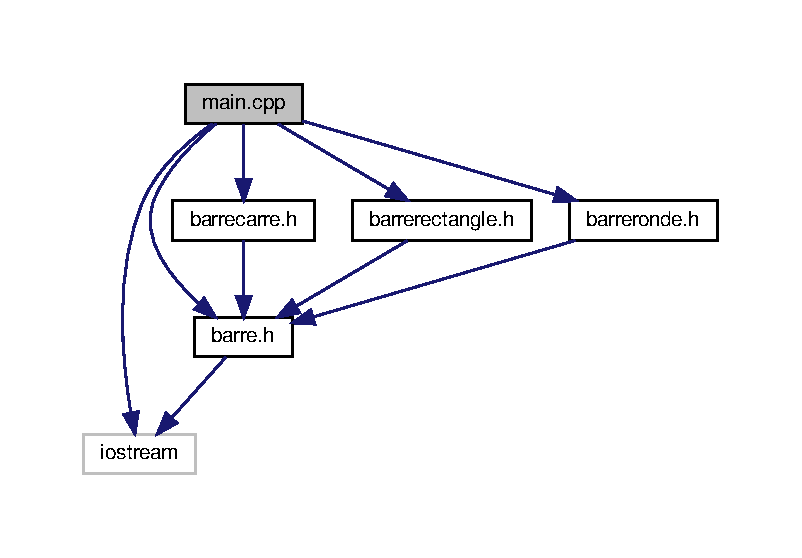
\includegraphics[width=350pt]{main_8cpp__incl}
\end{center}
\end{figure}
\subsection*{Fonctions}
\begin{DoxyCompactItemize}
\item 
int \hyperlink{main_8cpp_ae66f6b31b5ad750f1fe042a706a4e3d4}{main} ()
\end{DoxyCompactItemize}


\subsection{Documentation des fonctions}
\mbox{\Hypertarget{main_8cpp_ae66f6b31b5ad750f1fe042a706a4e3d4}\label{main_8cpp_ae66f6b31b5ad750f1fe042a706a4e3d4}} 
\index{main.\+cpp@{main.\+cpp}!main@{main}}
\index{main@{main}!main.\+cpp@{main.\+cpp}}
\subsubsection{\texorpdfstring{main()}{main()}}
{\footnotesize\ttfamily int main (\begin{DoxyParamCaption}{ }\end{DoxyParamCaption})}


%--- End generated contents ---

% Index
\backmatter
\newpage
\phantomsection
\clearemptydoublepage
\addcontentsline{toc}{chapter}{Index}
\printindex

\end{document}
